\section{Introduction}
In 2005, Jeff Howe and Mark Robinson created the term `Crowdsourcing' after a discussion about how businesses can outsource their work to individuals over the internet. There exist multiple definitions in the literature. Enrique Estell\'{e}s-Arolas and Fernando Gonz\'{a}lez Ladr\'{o}n-de-Guevara analysed over 40 definitions of crowdsourcing and developed a new integrating definition \cite{estelles}:\\\\
``Crowdsourcing is a type of participative online activity in which an individual, an institution, a non-profit organization, or company proposes to a group of individuals of varying knowledge, heterogeneity, and number, via a flexible open call, the voluntary undertaking of a task. The undertaking of the task, of variable complexity and modularity, and in which the crowd should participate bringing their work, money, knowledge and/or experience, always entails mutual benefit. The user will receive the satisfaction of a given type of need, be it economic, social recognition, self-esteem, or the development of individual skills, while the crowdsourcer will obtain and utilize to their advantage that what the user has brought to the venture, whose form will depend on the type of activity undertaken.''
\section{Platforms}
\subsection{Amazon Mechanical Turk}
The project was introduced in 2005 and is part of the Amazon Web Services\footnote{http://aws.amazon.com}. Requesters can post tasks known as HITs (Human Intelligence Tasks) which can be solved by workers (Amazon uses another term: Turkers). MTurk provides a web-based user interface and a couple of APIs in different programming languages (.NET, Java, Python, PHP, Perl, Ruby) to manage tasks. The first action of the requester is to create a HIT consisting of mandatory fields: 
\begin{itemize}
	\item \textbf{Title:} The requester must describe the idea of the HIT in at most 128 characters. 
	\item \textbf{Description:} A more detailed description of the task which cannot be longer than 2'000 characters. 
	\item \textbf{Question:} Every task has to contain questions to collect information from the crowd. The requester can decide between three question data structures. 
	\begin{itemize}
		\item \textit{QuestionForm}: The simplest form to create questions in a HIT. MTurk uses a special XML language to define tasks which has some restrictions. For example, JavaScript and CSS are not allowed. 
		\item \textit{ExternalQuestion}: MTurk will display a requester defined external webpage and the answers to the questions will be collected on the external website and send back to MTurk. This question data structure is used to overcome some restrictions of the platform like using JavaScript or to display CSS defined content. 
		\item \textit{HTMLQuestion}: This structure is a mixture between QuestionForm and ExternalQuestion. The requester has not to host an external website to provide a HTML based form. 
	\end{itemize}
	\item \textbf{Reward:} If the workers will successfully completing the HIT, then they will receive a predefined amount of money from the requester. 
	\item \textbf{Assignment duration in seconds:} The time in which the workers have to complete the task after they have accepted it. The time has to be between 30 seconds and one year. 
	\item \textbf{Lifetime in seconds:} The lifetime of a HIT defines the amount of time a task is acceptable for the workers. After the time elapsed, the HIT will no longer appear in the search results.
\end{itemize}
and some important, optional fields: 
\begin{itemize}
	\item \textbf{Keywords:} Comma separated keywords which describe the task (max. 2'000 characters). 
	\item \textbf{Max assignments:} Number of times a HIT can be completed. The default values is one. 
	\item \textbf{Qualification requirement:} Requesters can define requirements to process a task for the workers. For example, only workers who have more than 100 approved assignments can start working on a requesters HIT. 
\end{itemize}
After the tasks are designed, the requesters have to test them on the Amazon Mechanical Turk Developer Sandbox platform which is a simulated environment. If the requester is happy with the appearance of the HIT, the task can be published on the productive MTurk platform. Turkers have now the possibility to accept the HITs and complete the assignments until the lifetime is expired. After the HIT is completed, the requesters can take a look at the results and have to decide if they want to accept or reject the work. The workers will receive the predefined amount of money only for an accepted task. 

\subsection{Crowdflower}
A platform for large-scale data projects was founded in 2007. Crowdflower\footnote{http://www.crowdflower.com} has over 50 labor channel partners, Amazon Mechanical Turk for example, where the created tasks are published. The partner websites or communities are responsible to manage the registration and payment of their workers. The company offers enterprise solutions and enables a higher degree of quality control. `Gold standard data' (cf. \ref{sub:honeypots}, page \pageref{sub:honeypots}) and `Peer review' are two provided quality control techniques. `Peer review' gives the requesters the chance to improve the data by a second pass. A workflow management tool helps to link different jobs together. At the time of writing these lines, over one billion tasks are completed by workers domiciled in 208 different countries. Big companies like eBay use the Crowdflower service for their projects \cite{crowdflower_casestudy}. Over the past years, the company has completed over 15 projects. The improvement of the product categorisation algorithm was one of them.
\section{Patterns}
This section presents two probed ways to get useful information from the crowd.
\subsection{Find-Fix-Verify}
The Find-Fix-Verify pattern was introduced by the Soylent paper \cite{soylent}. The pattern divides the overall task into three stages. During the `Find' stage, the workers will identify patches of work done by the crowd or create new patches. For example, the workers have to select a sentence which seems to be incorrect and will need further investigations during the `Fix' phase. Some workers will revise the identified patches and try to provide alternatives. The last step of the pattern will present the generated alternatives during the `Fix' stage to a few new workers in a randomized order. The answer with the most votes (plurality voting) will be used to replace the identified patch during the first phase. The creators of the new suggestions will be suspended so that they cannot vote for their own input.

To illustrate the meaning of the Find-Fix-Verify pattern, the implementation of Soylent will be discussed (Figure \ref{fixfindverify}). The approach begins by splitting a text into paragraphs. During the `Find' stage, the workers have to identify candidate areas for shortening in each paragraph. If a certain number of workers have selected the same area, then this patch goes to the next stage. Every worker in the `Fix' stage has to present a shorter version of the identified patch if possible. They also have the possibility to say that the text cannot be reduced. During the last step, the crowd has to select rewrites which have spelling, style, or grammar problems or change the meaning of the sentence significantly. At the end, they remove these patches by a majority voting.
\begin{figure}[h!]
\centering
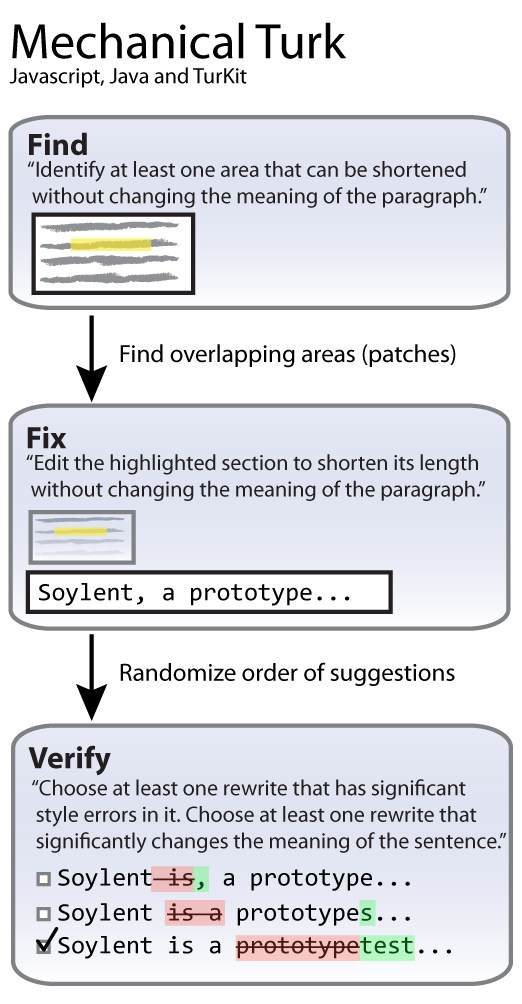
\includegraphics[scale=0.35]{images/soylent_system_overview.png}
\caption{Soylent Fix-Find-Verify pattern}
\label{fixfindverify}
\end{figure}

\subsection{Iterative}
\label{iterative}
Most of the published assignments on MTurk are independent, parallel tasks. However, also iterative sequential tasks can be useful. The authors of the TurKit paper \cite{turkit} implemented a tool which make iterative tasks possible. They developed an example application for creating an image description (Figure \ref{turkit}). During the first iteration, the worker will contribute the initial description of the provided image. The next iteration will show the initial description and a request to improve it. A few workers will evaluate the extension of the description by voting. If the extended description does not receive enough votes, then the iteration will be ignored. The final description is generated after a fixed number of iterations. To make the iterative solution possible, the crash-an-rerun programming model was introduced by the authors of the paper. This model allows a script to be re-executed after a crash without generating costly side-effects. This means, if there is a crash during the second iteration of an iterative problem, the first iteration will be skipped after re-running the script. TurKit is able to persist the state of the program and will never repeat successfully completed tasks. This is helpful for prototyping algorithms.
\begin{figure}
\centering
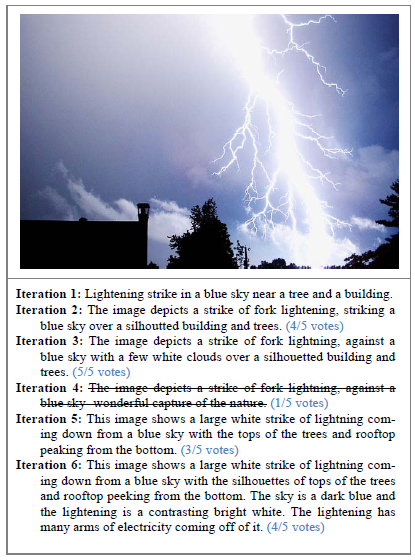
\includegraphics[scale=0.65]{images/turkit_description_example.png}
\caption{Iterative image description created by TurKit}
\label{turkit}
\end{figure}

\section{Design}
If requesters want to create new HITs, then they have to consider some design guidelines\cite{crowdsourcing_tutorial,mturk_bestpractices}: 
\begin{itemize}
\item \textbf{Be as specific as possible in the instructions:} If the requesters ask the workers ``Is a Ford Mustang a sports car?'', then this is not the same as they ask them ``Can a Ford Mustang accelerate from 0 to 100 km/h in 3 seconds or less?'' because the second one is clearer and more precise. Sometimes it is useful to hire a technical writer for phrasing task instructions. 
\item \textbf{Instructions have to be easy to read:} Instructions should be split into multiple subtasks and presented as a bulleted list. 
\item \textbf{Provide examples:} The best way to present the idea of a task is to show one or multiple examples. For example, this can help to avoid uncertainties if the instructions are misinterpreted or the workers have wrong expectations. 
\item \textbf{Mention what will not be accepted:} If a worker has to write a paragraph about an encyclopaedia article, the requester can allude in the instructions that copying contents from other website are prohibited.
\item \textbf{Tell the workers which tools they should use.} 
\item \textbf{Give the workers the possibility to write down a feedback about the task:} This is important to improve the design of the tasks, or can help to detect spammers. 
\item \textbf{Iterative and incremental development of tasks:} The first draft of a task will never be perfect. With the feedbacks and results of the previous iterations, the next one will contain improvements which should avoid foregoing mistakes or design failures.
\end{itemize}

\section{Hybrid}
A lot of information systems use a hybrid crowdsourcing technology. The combination of human intelligence and machine algorithms can lead to powerful information systems which cannot be realised by a pure machine approach. In most cases, the crowd is responsible to verify the created content of machine algorithms or to generate input data for them. 
A closer look at the CrowdSearch \cite{crowdsearch} project helps to illustrate the idea of hybrid systems. The developers implemented an image search system for cell phones. First, the system uses an automated image search to generate a set of candidate pictures. These are packed into multiple identical tasks for validation by humans and published on Amazon Mechanical Turk (Figure \ref{crowdsearch}). A simple majority voting is used to eliminating errors. After the validation of the results, the resulting image will be presented to the user. The drawbacks of such systems are that the hybrid approach generates additional costs for involving humans and the delay between publishing the tasks and receiving the corresponding results. The users of CrowdSearch can define a deadline before they query an image and the system will always return a result after the time is expired, irrespective of whether the crowdsourced tasks are completed or not. 
\begin{figure}
\centering
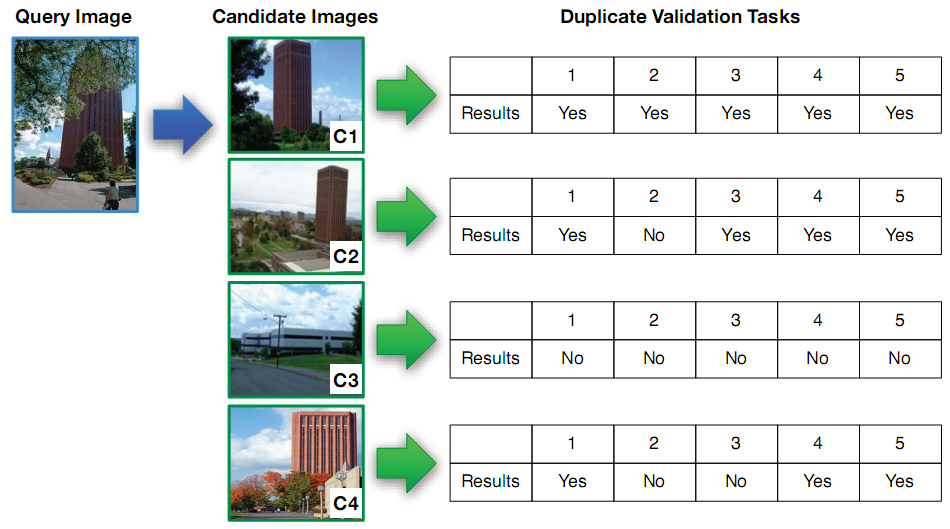
\includegraphics[scale=0.45]{images/crowdsearch_hybrid.png}
\caption{CrowdSearch hybrid image search approach}
\label{crowdsearch}
\end{figure}

\section{Quality Control}
Determination of the quality of completed tasks by the crowd is very important. Workers can be lazy or spammers who want to earn money for free or a minimal amount of work. To evaluate the performance of a single worker, several techniques are available. 
\subsection{Majority Voting}
To reduce the errors of single workers, majority voting can be used. If a majority has the same answer to a question, the requester can assume that the answer is correct. To break ties, an expert is necessary. 
\subsection{Honey Pots}
\label{sub:honeypots}
The requesters include trap questions where they know the correct answer. If the answer of a single worker is incorrect, the requester can exclude the results or reject the task. However, it is not always possible to generate honey pots. 
\subsection{Qualification Test}
MTurk provides the possibility to include a qualification test at the beginning of tasks. The worker has to pass the test to has access to the real tasks and the resulting rewards. The results of the test can be compared to an answer key automatically or by the requesters themselves. The additional effort and the determent of some workers are drawbacks of this procedure.

\section{Workflow}
A workflow is a set of tasks which are interconnected and easier to solve by the crowd. The output of a single subtask will be used for one or multiple subsequent subtasks. The output of the last element of the flow is the result of the entire complex task. There exists a lot of literature which covers the problematic of finding and interconnecting subtasks:\\\\
The process of decomposing complex tasks into simpler ones is not always easy and needs a lot of clarifications. The developers of the Turkomatic\cite{turkomatic} tool had an innovative idea and sourced the workflow decomposition out to the crowd. The workers have to decide how the final workflow should look like and what are the belonging tasks. The system consists of two major parts. The meta-workflow is used to design and execute workflows by applying the price-divide-solve (PDS) procedure. The workers have to recursively divide the complex task into smaller ones until they are simple enough. After this step, the workers will solve the generated tasks and other workers are asked to check the solutions. At the end, the results are combined into a cohesive answer. The second part of the Turkomatic system allows a visualisation of the created workflows and an edit function to manually adapt the crowdsourced results.

Another idea was pursued by the developers of CrowdForge\cite{crowdforge}. They designed a framework to create a workflow by using several partition, map and reduce steps. The partition step splits a larger task into smaller subtasks, the map step lets one or more workers process a specified task. The results of the workers are merged into a single output during the reduce step. For example, the workers should write an encyclopaedia article about a given topic (Figure \ref{crowdforgeflow}). The authors of the paper solved this problem by the presented partition/map/reduce steps. First, the partition step asks the workers to create an outline of the article by defining section headings (e.g. ``History'', ``Geography''). During the map phase, multiple workers are asked to provide a single fact about the section (e.g. ``The Empire State Building celebrated its 75th Anniversary on May 1, 2006'' if it is an encyclopaedia article about ``New York'' and the section heading is ``Attractions''). The workers have to piece the collected facts together to a completed paragraph during the reduction step.

The CrowdForge prototype is written in Python using the Django\footnote{https://www.djangoproject.com} web framework and boto\footnote{https://github.com/boto/boto}, an interface to the Amazon Web Services which is available in Python. The user can define complex flows by creating HIT templates (which can be either a partition, map or reduce task) and dependencies between the templates. Flows are implemented as Python classes. The prototype is also responsible for the sequential coordination between the HITs (including data transfer). Multiple independent flows can be executed simultaneously. One of the limitations is that CrowdForge does not support iteration or recursion. The further development of the project was suspended in 2011.

The same crew developed CrowdWeaver\cite{crowdweaver} which is an advancement of the CrowdForge project. They use CrowdFlower, another crowdsourcing platform, instead of Amazon Mechanical Turk. On CrowdFlower, the requesters can create tasks on multiple markets (including MTurk). Flows can be created visually and does not assume any programming skills. Another feature is the tracking and notification of crowd factors, for example latency or price.
\begin{figure}
\centering
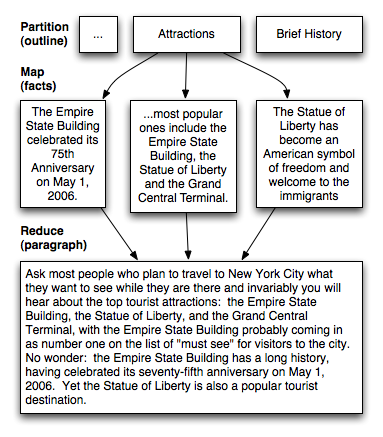
\includegraphics[scale=0.6]{images/crowdforge-article.png}
\caption{CrowdForge example workflow}
\label{crowdforgeflow}
\end{figure}
\section{Incentives}
There are multiple aspects which motivate users to contribute their human power and knowledge. Some of them are described in the following lines.
\subsection{Gamification}
The ESP game\cite{esp} makes the labelling of any kind of images in the web possible. There are no guidelines to provide images and no computer vision method exists which can handle the diversity of all images. Search engines are dependent on accurate image descriptions to represent relevant results. Therefore, another approach was introduced by the article. An online, web-based game was developed to attract workers. Two players are randomly assigned to label the same image simultaneously. There is no possibility to communicate with the game partner. Each player has to guess the description of the image independently without uses the `Taboo words'. These words are evaluated by a prior round and will be ignored for the actual turn. If there is a match between both players, the score will be increased and another image description is detected. The discovered word will only be taken as a valid description and `Taboo word' if a predefined number of players had the same agreement. The duration of the whole game is 150 seconds and both parties can guess as many images as possible within this time. 
During the period of four months, the game was played by 13'630 people and 1'271'451 labels for 293'760 images were generated. These numbers show the power of the idea. The players (crowd) did not know what is going on behind the scenes and they also did not realise the purpose of their inputs.

\subsection{Socialisation}
``Social factors such as the desire to feel a sense of involvement and `belong' to a social group, and the forming and maintaining of interpersonal bounds, are a fundamental human need. Empirical studies also show that social motivation is an important driver for people taking part in online activities, ranging from knowledge contribution to providing emotional support.'' \cite{yu} \\
\\
One example project which use this social incentive is `stackoverflow'\footnote{http://stackoverflow.com/}. People are able to post questions about computer programming issues and other users will provide their help for free. Good answers will receive votes from other contributors and the person who asked the question is authorised to mark an answer as accepted. Hard workers can earn reputation points from other users for questions, answers or edits. A higher reputation score will unlock advanced functionalities. Another way to earn respect from other users is to gather badges. These are achievements which are available in three levels: bronze, silver and gold. ``Answer score of 100 and more'', ``Asked a question with 10'000 views'' or ``Visited the site each day for 30 consecutive days'' are example activities which will be rewarded with badges. The two presented rewards motivate the users of the website to contribute as much content as possible. The community itself is controlling the quality of the answers because experts can remove wrong or low quality statements. Normal users can penalise improper answers by not voting for them. The service sorts answers based on the votes in descending order and the worst evidences will be ignored by the customers.

\subsection{Unintended by-product}
Data from the crowd is collected as an involuntary by-product of the main purpose. One of the most famous projects is reCAPTCHA\cite{recaptcha} which is a further development of the well known Captcha\footnote{http://www.captcha.net/} idea. The method will show distorted characters, which cannot be recognised by the OCR (Optical Character Recognition) software, to the internet users. The reCAPTCHA acts like a normal Captcha but the inputs will be used additionally to improve text recognition systems.

Another project from the same inventor is Duolingo\footnote{https://www.duolingo.com}. Luis von Ahn has the vision to translate every page in the web into all major languages. He hides the main purpose of the service behind a free foreign language learning program. Companies remunerate the founder of the project for translated documents.

\subsection{Financial Reward}
Another possibility to attract workers is the good old money. Crowdsourcing platforms offer to pay them for accepted tasks. If the payment is too low, then workers will not process the tasks. High rewards will attract spammers who deliver bad quality work to collect as much cash as possible in a short amount of time. A research paper from Yahoo \cite{mason} investigates the relationship between financial reward, and the performance of the crowd. They found out, that a higher payment increases the quantity of the work and not it is quality. They proposed to use other incentives like enjoyable tasks or social rewards because the quality of work is the same or better than financial driven approaches. A second advice is that requesters should use as less money as possible only if a payment of the workers is possible. Based on the fact that work will be done faster but not better if a higher gratification will be paid.

Amazon itself does not provide numbers but suggests to take a look at similar HITs to compare rewards \cite{mturk_bestpractices}. A good strategy is also to proof how long it takes to complete the own tasks and then calculate how many tasks can be done in one hour. Different analyses \cite{chilton,ipeirotis} show that the median wage is \$1.38/hour and the average wage \$4.8/hour. The Mechanical Turk Tracker website\footnote{http://mturk-tracker.com} was developed by the author of one of these statistics \cite{ipeirotis} and it is possible to calculate the average cost per HIT for a specific day. On 10th of March 2014, the website tracked 236'370 completed HITs with a total reward of \$23'110 and an average of \$0.097/HIT. These numbers should help the requesters to find an initial price for their tasks. However, there is no general formula to calculate the right costs for an HIT. If the initial price is too low, the workers will ignore those tasks and try to find others with a better revenue/expense ratio. This results in higher completion times. In this case, the requesters should increase the reward. On the other side if the tasks will be completed very fast and the results are not like expected, then a decrease of the reward can be helpful.

\section{Demography}
The workers on the MTurk platform are hidden behind an identification number, no details about gender or country of residence are available. To get detailed information about the workers, researchers from the University of California published surveys in the form of HITs\cite{ross} and presented their results in 2010. They observed the crowd for about 20 months and detected some changes over time. The number of Indian workers raised significantly within one year and approximately one third of the workers were from there. The majority of the turkers was located in the United States (56\%) and every tenth in the United Kingdom, Canada or Philippines. The distribution between female and male participants was nearly equal and most of them were between 18 and 35 years old. A very interesting fact is that 41 percent of the workers were highly educated (Bachelor degree). The authors of the paper also provided numbers about the financial situations of the crowd. A fifth needed the money to always or sometimes make basic end meets, 30 percent to buy for nice extras. 
Unfortunately, the presented facts are four years old but no current numbers are available for the Amazon Mechanical Turk platform.

